\documentclass[parskip,
							 oneside,
% 							 longdoc,
							 11pt,
							 noheadingspace,
							 accentcolor=tud1d,
							 bigchapter,
							 %draft,
							 colorback]{tudreport}


%% Spracheinstellungen
\usepackage[ngerman]{babel}
%\usepackage[applemac]{inputenc} % Input-Encodung: applemac fuer Mac
%\IfFileExists{latin1.sty}{\usepackage{latin1}}{\usepackage{isolatin1}}
%\usepackage[latin1]{inputenc}
%\usepackage[T1]{fontenc}
\usepackage[ansinew]{inputenc}  % Input-Encodung: ansinew fuer Windows
\usepackage{microtype} % optischer Randausgleich bei pdflatex mit Zeichendehnung
\usepackage{caption}
\usepackage{graphicx}

%% Grafikeinstellungen
\usepackage{float} % u.a. genaue Plazierung von Gleitobjekten mit H
%\usepackage[latin1]{inputenc}


%% Tabelleneinstellungen
\usepackage{booktabs}
\usepackage{multirow}
\usepackage{longtable}
\usepackage{tabularx}

%% State Chart
\usepackage{pgf}
\usepackage{tikz}
\usetikzlibrary{arrows,automata}

%% Mathematik
\usepackage{amsmath}
\usepackage{nicefrac}
\usepackage{icomma}

%% sonstige Einstellungen
\usepackage{paralist}% erweiterte Listenumgebung (z.B. compactitem)
\usepackage{textcomp} % verschiedene Symbole
\usepackage[nottoc, numbib]{tocbibind}
\usepackage{hyperref}
\renewcommand\plparsep{1ex}
\usepackage{enumerate}
\usepackage{listings}
\usepackage{color}

\definecolor{dkgreen}{rgb}{0,0.6,0}
\definecolor{gray}{rgb}{0.5,0.5,0.5}
\definecolor{mauve}{rgb}{0.58,0,0.82}

\lstset{frame=tb,
  language=Java,
  aboveskip=3mm,
  belowskip=3mm,
  showstringspaces=false,
  columns=flexible,
  basicstyle={\small\ttfamily},
  numbers=none,
  numberstyle=\tiny\color{gray},
  keywordstyle=\color{blue},
  commentstyle=\color{dkgreen},
  stringstyle=\color{mauve},
  breaklines=true,
  breakatwhitespace=true,
  tabsize=3
}

\title{\textbf{Projektseminar Rechnersysteme}}
\subtitle{Seminararbeit vorgelegt von (Robert Wiesner)}
\subsubtitle{Betreuer: Dipl.-Ing. (Changgong Li)\\
			 Beginn: (Beginndatum) \textbar\ Abgabe: (Abgabedatum)\\
			 Institut f\"ur Datentechnik\hfill\textbar\hfill Fachgebiet Rechnersysteme\hfill\textbar\hfill Prof.\,Dr.-Ing.\, Christian Hochberger}
\setinstitutionlogo{images/logo.pdf}
% \institution{Institut f\"ur Datentechnik\hfill\textbar\hfill Fachgebiet Rechnersysteme\hfill\textbar\hfill Prof.\,Dr.-Ing.\, Hans Eveking}
%\settitlepicture{images/spartan}
\begin{document}
%% Titel %%%%%%%%%%%%%%%%%%%%%%%%%%%%%%%%%%%%%%%%%%%%%%%%%%%%%%%%%%%%%%%%%%
\maketitle
\cleardoublepage

%% Vorgeplnkel %%%%%%%%%%%%%%%%%%%%%%%%%%%%%%%%%%%%%%%%%%%%%%%%%%%%%%%%%%%%%%
\pagestyle{empty}
%\pagenumbering{roman}


%% Hauptteil %%%%%%%%%%%%%%%%%%%%%%%%%%%%%%%%%%%%%%%%%%%%%%%%%%%%%%%%%%%%%%%
\pagestyle{headings}
\pagenumbering{arabic}
\tableofcontents 
\chapter{Aufgabenstellung}
\label{cha:Aufgabenstellung}

Entwicklung eines Spill and Fill Mechanismus um den Framestack des AMIDAR Prozessors auf einen externen DDR3 Speicher auszulagern und so die maximal m�gliche Stackgr��e deutlich zu erh�hen. Dazu geh�rt das einrichten verschiebbarer "windows", die jeweils einen Ausschnitt des Stacks beinhalten. 
Bei einem Methodenaufruf, dessen Stackframe den aktuellen Ausschnitt �berschreiten w�rde, soll ein Teil der im Window enthaltenen Daten auf den externen Speicher ausgelagert werden, um Platz f�r den neuen Stackframe zu schaffen. Bei einem Methoden R�cksprung sollen die Daten wieder zur�ck kopiert werden um den alten Stackframe wiederherzustellen. 
Es sollen 4 Windows angelegt werden um die Stacks von bis zu 4 Threads vorzuhalten. Es soll die M�glichkeit einer Threadverdr�ngung realisiert werden, damit mehr als 4 Threads ausgef�hrt werden k�nnen. 




\chapter{Grundlagen}
\label{cha:Grundlagen}

\section{AMIDAR }
Bei der Klasse der AMIDAR Prozessoren handelt es sich um ein konfigurierbares System, bestehend aus Function Units (FU). Komplexe Instruktionen werden in mehrere Arbeitsschritte unterteilt, die als Token an die einzelnen FUs verteilt werden. Daf"ur wird das Token Distribution Network genutzt. F"ur die Kommunikation zwischen den FUs, gibt es auch noch einen Datenbus. Ein Vorteil der AMIDAR Architektur ist, dass leicht FUs eingef"ugt werden k"onnen, um den Prozessor an die Aufgaben anzupassen. Ein gutes Beispiel daf"ur sind die Hardwarebeschleuniger. \cite{Burkert}\cite{Andresen}

\begin{figure}[H]
	\centering
	\includegraphics[height = 7cm]{PS_RS_graphics/AMIDAR.pdf}
	\caption{AMIDAR}
\end{figure}

\subsection{Lokale Variablen und Operanden in Java}
Java ist ein Objektorientierte Programmiersprache. Programme die in Java geschrieben worden sind, werden "ublicherweise in einer virtuellen Maschine ausgef"uhrt. 
Dabei werden Frames genutzt, die f"ur die Ausf"uhrung einer Methode wichtige Daten beinhalten. Ein Frame wird bei einen Methodenaufruf erzeugt und bei einen Methodenr"ucksprung zerst"ort. Ein Frame enh"alt jeweils den Speicher f"ur die lokalen Variablen, wie auch den Operandstack.  
Die Java Virtual Machine arbeitet Stackbasiert, was bedeutet, das Operanden nicht, wie in einer Registermaschine, in Registern gespeichert werden, sondern auf den Operandstack gelegt werden. Rechenoperationen und Funktionsaufrufe nehmen jeweils die obersten Werte des Operandstacks als Parameter. 

\subsection{Framestack}
Die AMIDAR Implementierung, die am Fachgebiet Rechnersysteme entwickelt wird, arbeitet mit Java Bytecode. Dabei wird der Stack f"ur Lokale Variablen und der Operandenstack in der Framestack FU zusammengefasst. Durch das Zusammenfassen beider Stacks, werden Kopiervorg"ange "uber den AMIDAR Bus eingespart. Zum einen m"ussten lokale Variablen bei jeder Verwendung auf den Operandstack kopiert werden, zum anderen m"ussten Parameter bei jeden Funktionsaufruf in den lokalen Variablenspeicher kopiert werden.
Der AMIDAR Framestack arbeitet bei der Stackframe Verarbeitung mit drei grunds"atzlichen Zeigern. Der Stackpointer gibt die n"achste freie Speicheradresse "uber den aktuellen Stackframe an. Der Locals Pointer gibt die unterste Lokale Variable und damit auch das untere Ende des Stackframes an. Der dritte wichtige Zeiger ist der Callercontext Pointer, der auf die unterste Adresse des Callercontext deutet. \cite{Illy}

\subsubsection{Stackframe}
Ein Stackframe beginnt mit den Parametern und den Lokalen Variablen.  Dar"uber kommt der Callercontext mit den alten Localspointer, Stackpointer und Callercontextpointer. Das obere Ende des Stackframes besteht aus dem Callercontext. 
\cite{Illy}

\subsubsection{Funktionsaufrufe}
\begin{figure}[H]
	\centering
	\includegraphics[height = 10cm]{PS_RS_graphics/StackframebeforeInvoke.pdf}
	\caption{Stackframe vor einen Funktionsaufruf}
\end{figure}
Eine f"ur dieses Projekt wichtige Funktion des Framestacks sind Funktionsaufrufe. Bei einen Funktionsaufruf werden im Framestack die 3 wichtigen Pointer neu gesetzt, wobei die alten Werte im Callercontext gesichert werden. Der neue Localspointer wird berechnet, in dem vom aktuellen Stackpointer die Anzahl der Parameter, der aufgerufenen Methode, abgezogen wird. Der neue Callercontextpointer wird berechnet, indem auf dem neuen Localspointer, die mit den Token "ubergebene, Anzahl lokaler Variablen addiert wird. Der neue Stackpointer wird berechnet, in dem auf dem Callercontextpointer die gr"o"ze des Callercontext addiert wird. 
In den n"achten Takten werden die alten Localspointer, Stackpointer und Callercontextpointer in den Callercontext geschrieben. \cite{Illy}
\begin{figure}[H]
	\centering
	\includegraphics[height = 10cm]{PS_RS_graphics/StackframeafterInvoke.pdf}
	\caption{Stackframe nach einen Funktionsaufruf}
\end{figure}


\subsubsection{Funktionsr"ucksprung}

Bei einem Funktionsr"ucksprung werden im AMIDAR Framestack die Locals- Stack- und Callercontextpointer aktualisiert. Der Vorgang beginnt, wenn eines der entsprechenden Token "uber den AMDIAR Bus gesendet wird. Es gibt 3 Varianten des Tokens. Eine liefert keinen R"uckgabewert, die anderen geben jeweils 32 oder 64 Bit zur"uck. Wenn der Token abgearbeitet wird, werden nacheinander die drei Pointer ausgelesen und wiederhergestellt. Anschlie"zend wird gegebenenfalls der R"uckgabewerte gesichert, dieser steht in den top of Stack bzw. next of stack Registern. Der R"uckgabewert wird an Stelle des obersten, im Falle eines Return64 der oberen beiden, Operanden des Urspr"unglichen Funktionsaufruf gespeichert. \cite{Illy}

\begin{figure}[H]
	\centering
	\includegraphics[height = 10cm]{PS_RS_graphics/Stackframeafterreturn.pdf}
	\caption{Stackframe nach einen Funktionsr"ucksprung}
\end{figure}
\section{Spill and Fill}

Spill and Fill beschreibt eine Strategie, durch die der Zugriff auf einen Stapelspeicher deutlich beschleunigt werden kann. Ein kleinerer, schnellerer Speicher h"alt einen Ausschnitt des Hauptspeichers vor, der je nach Bedarf hoch oder runter geschoben werden kann, sodass immer das obere Ende des Stapelspeichers im Window Ausschnitt liegt. Spill beschreibt dabei den Vorgang des nach oben Schiebens des Speicherausschnitts, bei den der untere Abschnitt des Ausschnitts in den Hauptspeicher geschrieben wird. Wird der Stack weit genug abgebaut, wird ein Fill durchgef"uhrt, bei dem die ausgelagerten Teile zur"uck kopiert werden.  

\begin{figure}[H]
	\centering
	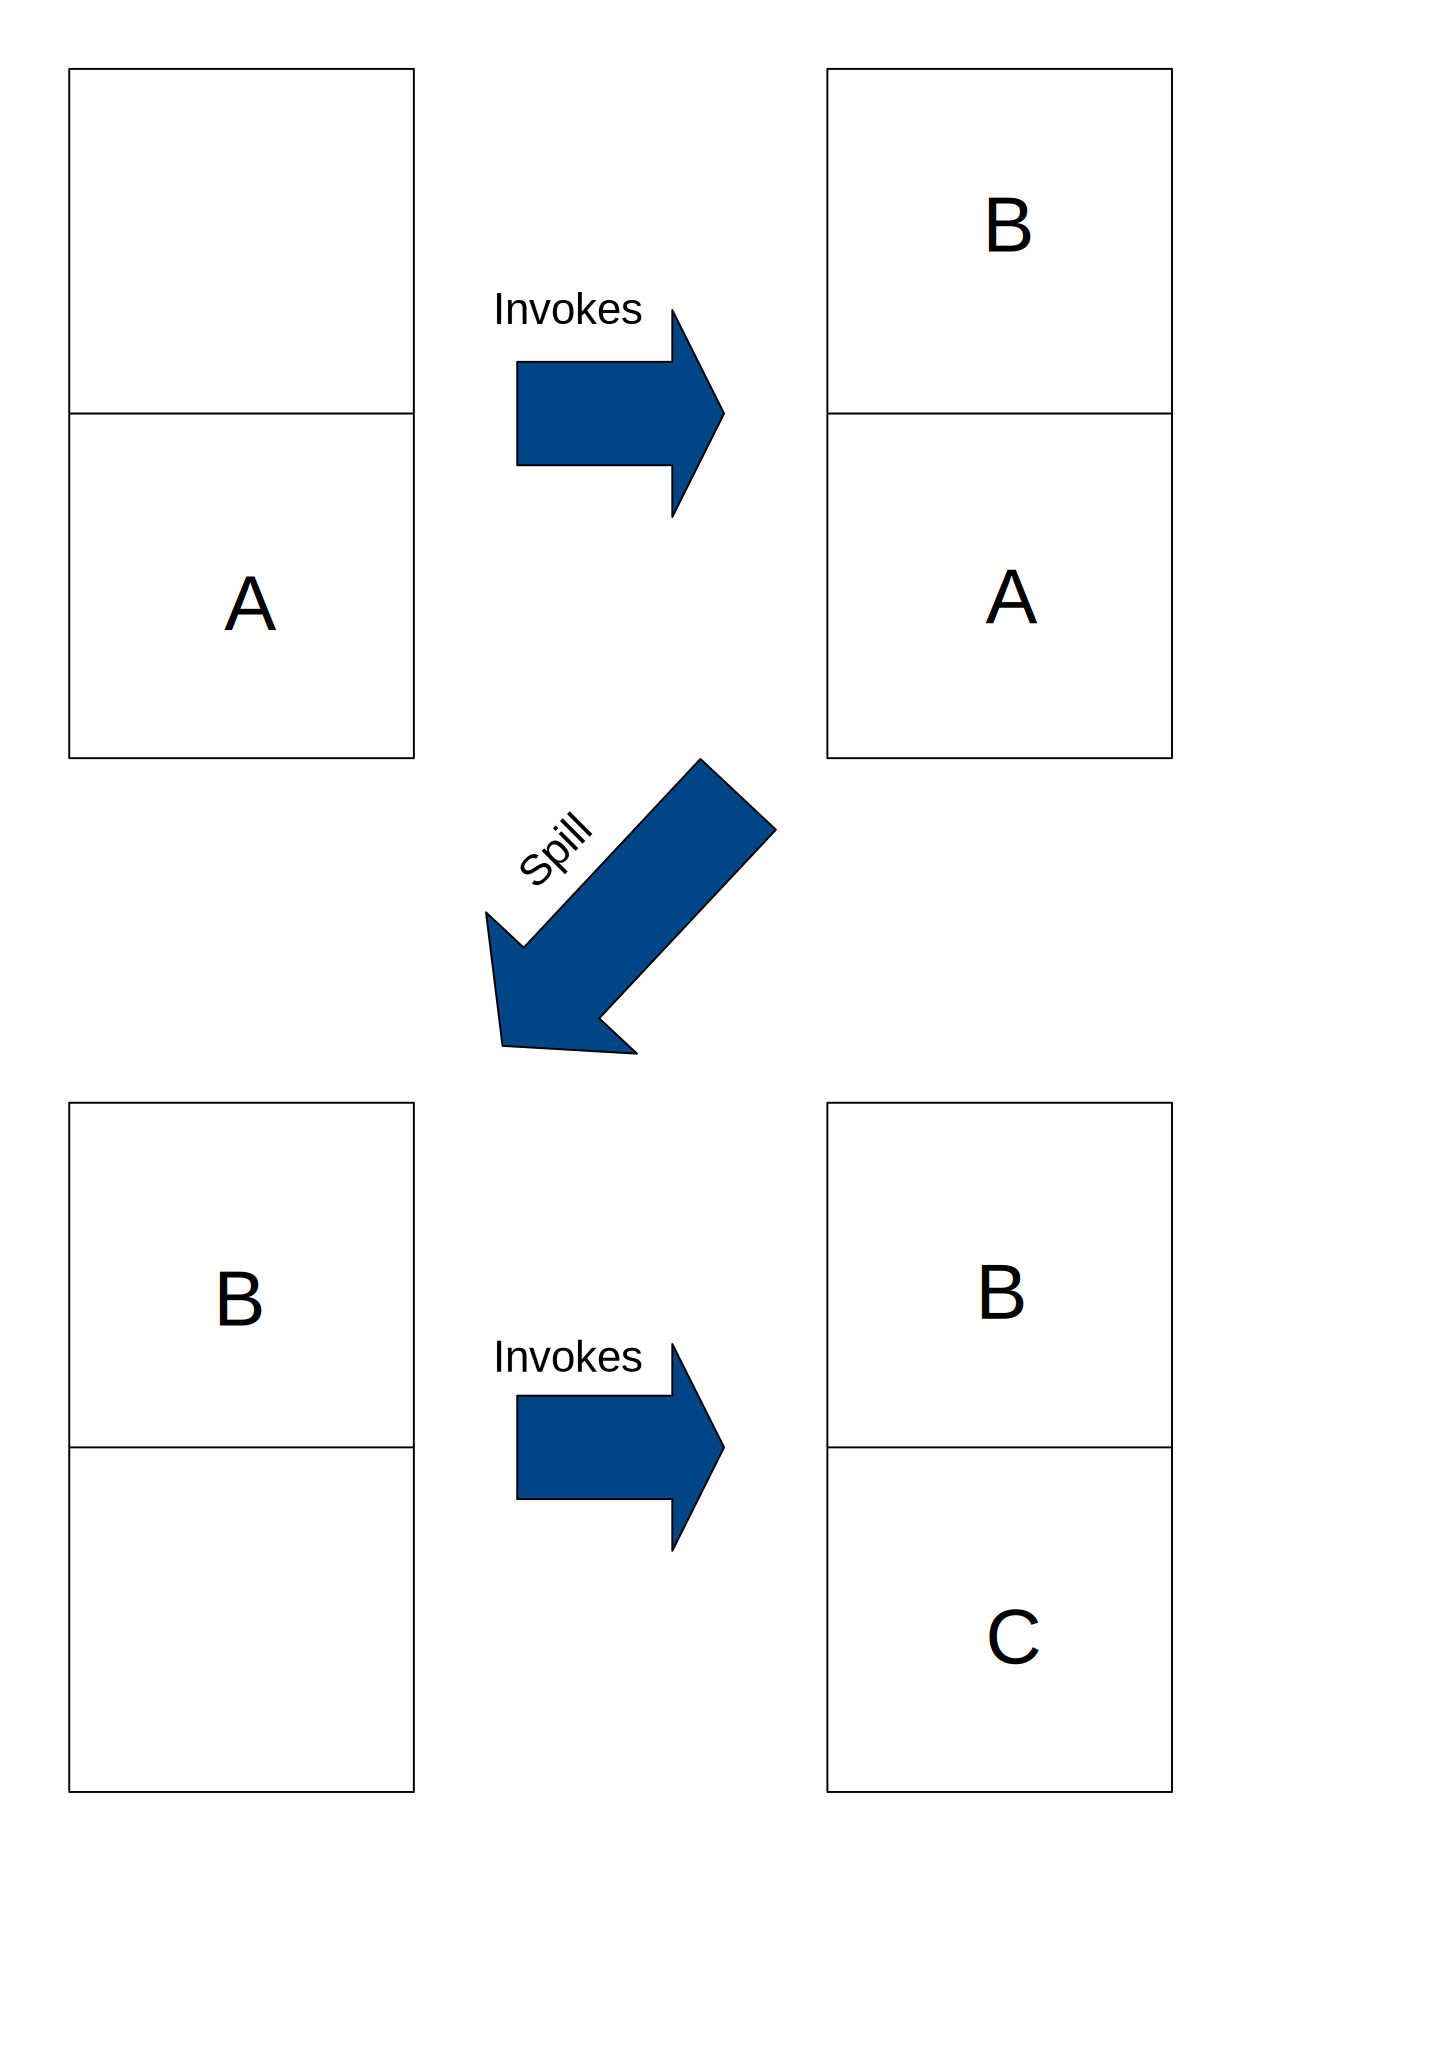
\includegraphics[height = 10cm]{PS_RS_graphics/spill.pdf}
	\caption{Spill: Verschieben des Windows }
\end{figure}

\begin{figure}[H]
	\centering
	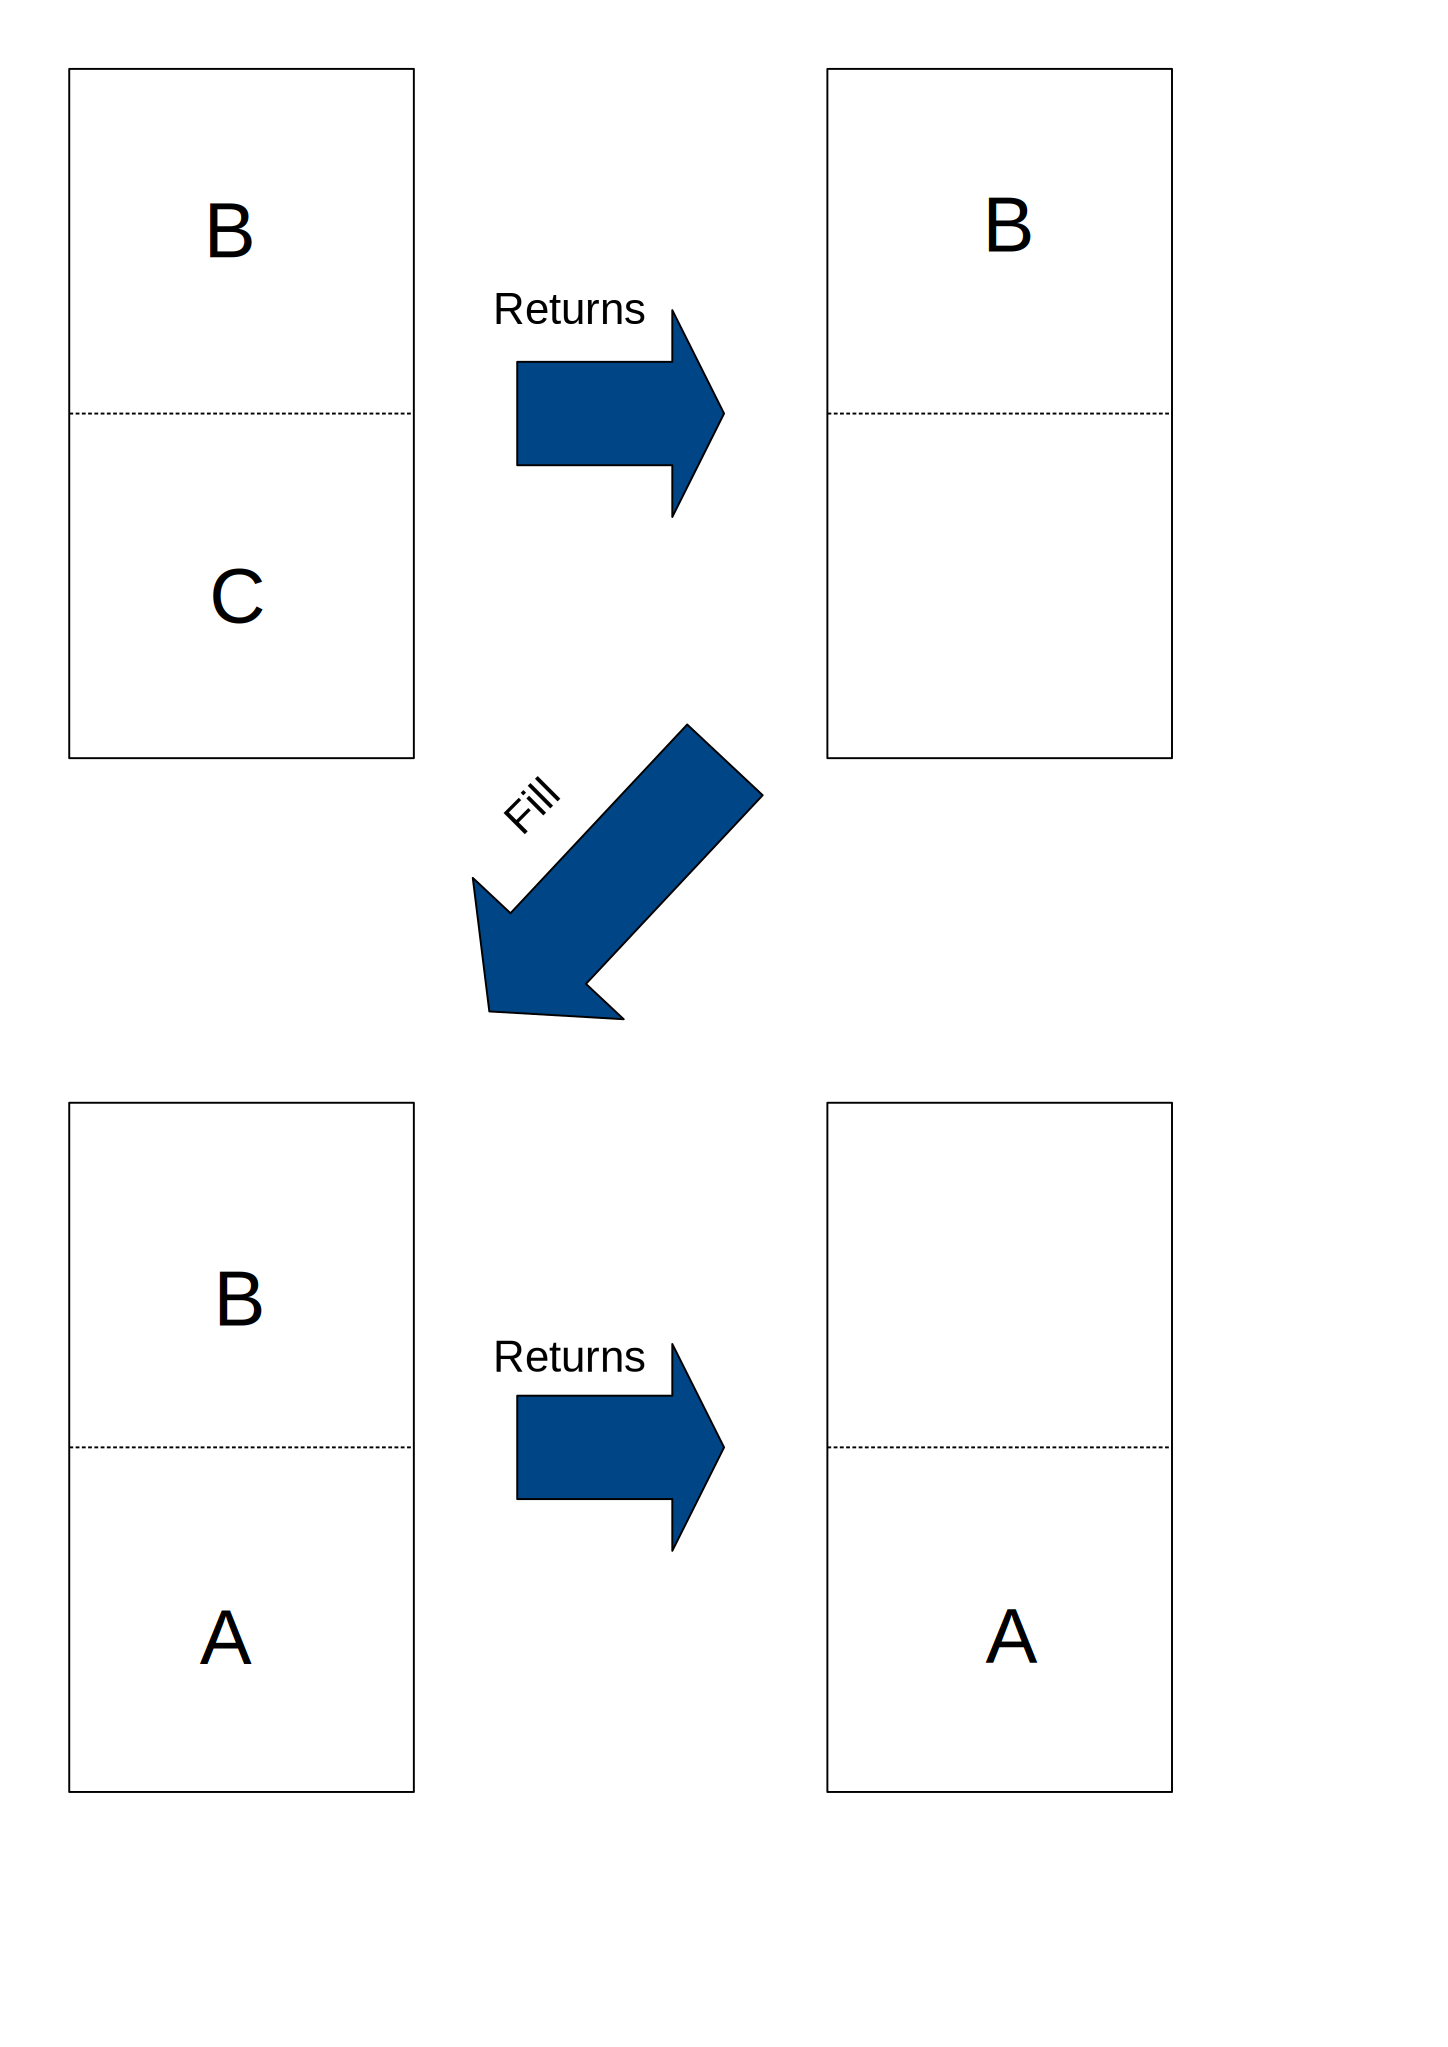
\includegraphics[height = 10cm]{PS_RS_graphics/fill.pdf}
	\caption{Fill: Verschieben des Windows}
\end{figure}


\begin{minipage}{\linewidth}
\section{Verwendung eines Spill and Fill Mechanismus in anderen Prozessoren}
\subsection{Sun Sparc Prozessoren}
Die Sun Sparc Prozessoren V8/V9 verf\"ugen \"uber ein sliding register Window mit jeweils 16 64 Bit gro"zen Registern in 7 Registers\"atzen. Sliding Window bezeichnet ein Verfahren, bei dem die Registers\"atze im Falle eines Funktionsaufruf nicht auf dem Stack gesichert werden m\"ussen, stattdessen wird auf den n\"achsten Registersatz gewechselt. Dabei wird meistens auch die Parameter\"ubergabe realisiert. Dabei sind die Input Register in dem Registerwindow des Callers identisch mit dem Output Registern, in dem Registerwindow des Callee.   
Mit speziellen Bytecode Instruktionen werden im Spill an Fill Verfahren Registers\"atze auf einen externen Speicher gesichert. Da das Spill and Fill durch spezielle Bytecodes ausgel"ost wird muss der Compiler vorher festlegen an welchen Stellen im Programm das Spill and Fill stattfinden soll. \cite{Gove}
\end{minipage}
\chapter{Implementierung}
\label{cha:Implementierung}
\section{DRAM Anbindung \"uber AXI}
AMIDAR ist \"uber AXI mit 512 MB DDR Ram verbunden, der auf 800 MHz getaktet.


\subsection{Addressbereich des Framestacks im Hauptspeicher}
Eine Schwierigkeit bei der Auslagerung des Framestacks an den Hauptspeicher ist die Unterschiedliche Wortbreite. 
F\"ur den Garbarbagecollector werden zu jedem 32bit Datenwort noch 2 Statusbit gespeichert in den festgehalten wird, ob es sich bei den Daten um Metadaten, Referenzen oder Werte handelt. Damit beim Auslagern der Daten auf dem externen Speicher diese Informationen nicht verloren gehen werden die Schreibvorg\"ange immer in Bl\"ocken von 16 W\"ortern durchgef\"uhrt, wobei die Statusbits der 16 W\"orter als weiteres 32Bit Wort in den Speicher geschrieben werden. Dies ist kein Problem, da die Gr\"o"se der beim Spill and Fill Vorgang \"ubertragenen Bereiche einen Vielfachen von 16 W\"ortern entspricht. 

\begin{figure}
	\centering
	\includegraphics[height = 15cm]{PS_RS_graphics/FS Blocks in Ram.pdf}
	\caption{Zuordnung der Framestack Adressen im Hauptspeicher}
\end{figure}

Der Ausgelagerter Framestack wird in das obere Ende des 512MB großen DDR3 Speicher gelegt und belegt:\\ $(number max threads * words per thread)*(1+1/16) $ W"orter.\\
Als Ausgangspunkt wird die h"ochste Speicheradresse des DDR Speichers verwendet und 2 mal nach links geshiftet, da der externe Speicher Byte adressiert, der Framestack jedoch wortadressiert ist. Davon wird die Maximale Gr"o{\ss} des Framestacks abgezogen. Von da an aufw"arts werden die Daten der einzelnen Threads gespeichert.

\subsection{Schreiben von Framestackinhalten in den Hauptspeicher}
F\"ur das Zwischenspeichern und packen der Bl\"ocke wird ein eigenes Modul verwendet.
Vom Framestack aus kann auf dieses Modul geschrieben werden. Dabei wird die Startadresse des Blocks, die l"ange des AXI Bursts und das erste Datenwort angelegt. Zum Zwischenspeichern dieser Daten werden jeweils Fifos verwendet. Wobei die Fifos f"ur Burstl"ange und Startadresse einen Sechzehntel der Gr"o{\ss}e des Datenfifos haben. F"ur jedes "ubertragene Datenwort werden 2 Statusbits in einen 32 Bit Register geschrieben. Nach dem 16 Datenworte in den Datenfifo geschrieben wurden wird der Inhalt dieses Registers in den Fifo geschrieben. 
Das Modul, indem die eigentliche AXI "Ubertragung verarbeitet wird wartet darauf das der Adress- und Burstlengthfifo nicht leer sind. Wenn die der Fall ist wird die Adresse und Burstl"ange ausgelesen und wie folgt umgerechnet:

Anschlie{\ss}end werden die Daten aus dem Fifo \"ubertragen bis die neu berechnete Burstl"ange erreicht wurde. Solange der noch Eintr\"age in den Fifos f"ur Bursl"ange und Adresse liegen wird eine neue "Ubertragung gestartet. 

\begin{figure}
	\centering
	\includegraphics[height = 15cm]{PS_RS_graphics/Axi Write Buffer.pdf}
	\caption{Schema des AXI Schreib Puffers}
\end{figure}

\subsection{Lesen von Framestackinhalten aus den Hauptspeicher}
Wenn die Daten ausgelesen werden sollen, wird das selbe Modul verwendet. Es wird die Startadresse des auszulesenden Blocks und die Burstl"ange \"ubergeben. Diese wird f\"ur den DDR Speicher umgerechnet und der Lesevorgang \"uber AXI gestartet. F"ur das Zwischenspeichern der ausgelesenen Daten werden  Das erfolgreiche Einlesen wird dem Framestack signalisiert, woraufhin die Daten des Blocks ausgelesen werden. Zum Zwischenspeichern der ausgelesenen Daten werden 2 Fifos verwendet. Ein Fifo wird f"ur die gelesenen Daten speichert 32 W"orter mit 32 Bit Wortbreite. In einen weiteren Fifo ebenfalls 32Bit werden die kumulierten Statusbits gespeichert. Nachdem die ersten 16bit Datenworte in den Fifo gespeichert wurden, enth"alt das n"achste Wort die Statusbits, dieses wird in den entsprechenden Fifo gespeichert. Sobald das Fifo f"ur die Statusbits nicht leer ist, kann auf Seiten des Framestacks mit den Auslesen begonnen werden. Bei jeden takt in dem eine 1 an readenable angelegt ist wird ein Datenwort aus dem Fifo und 2 Statusbits "ubertragen. Nach dem 16 W"orter aus den Datenfifo gelesen wurden wird wenn vorhanden das n"achste Statuswort aus den Statusfifo gelesen. 

\begin{figure}
	\centering
	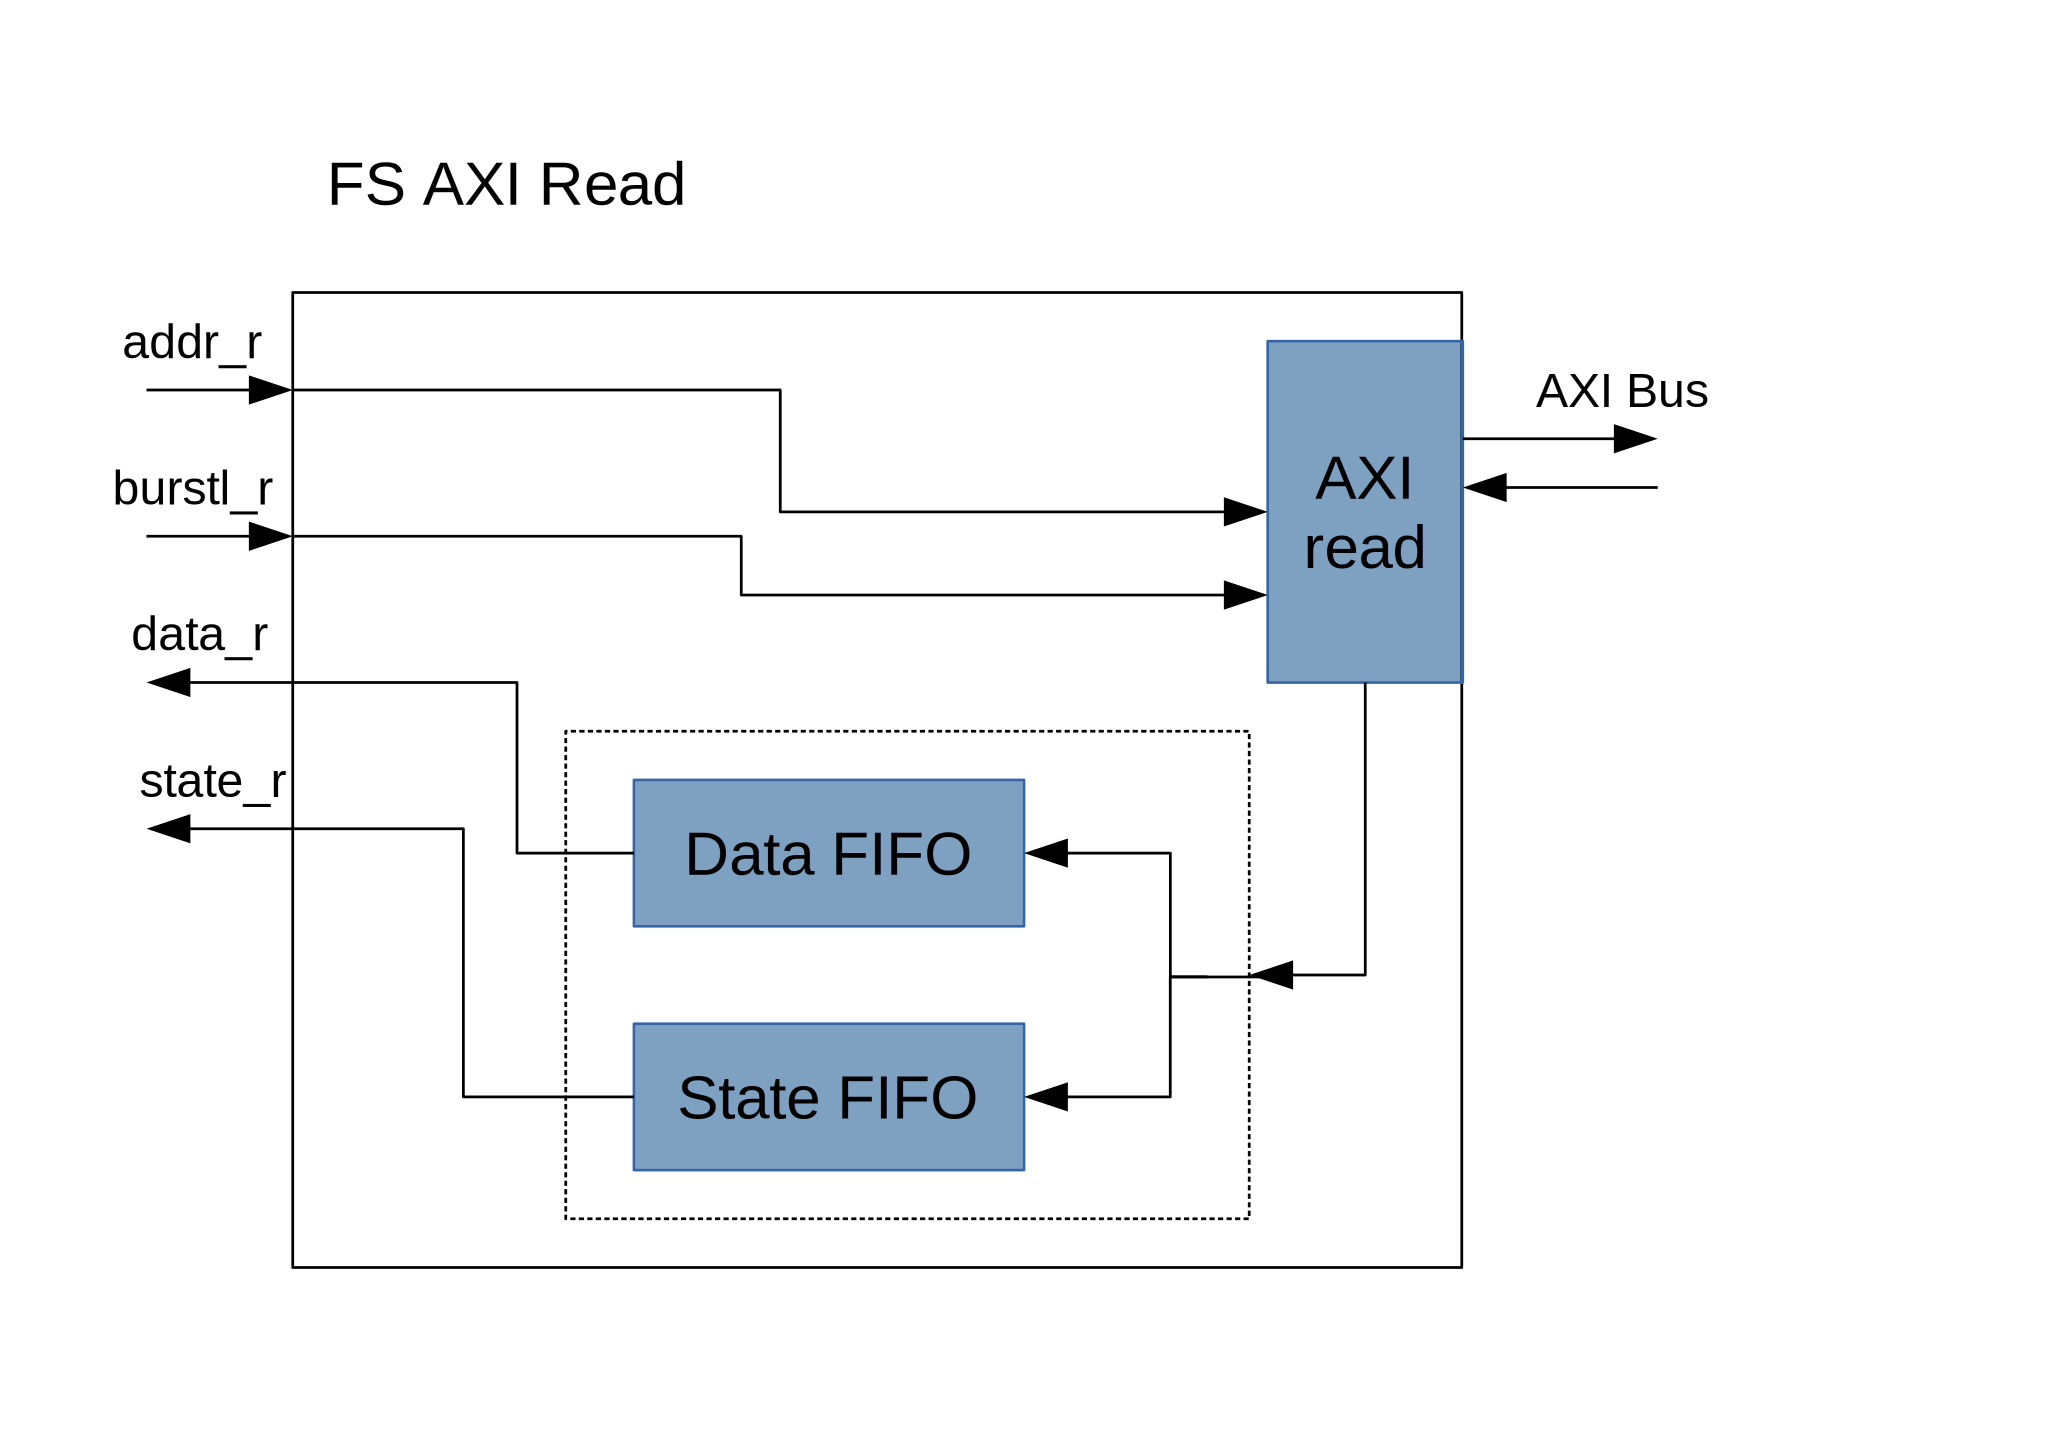
\includegraphics[height = 15cm]{PS_RS_graphics/Axi Read Buffer.pdf}
	\caption{Schema des AXI Lese Puffers}
\end{figure}

\section{Spill and Fill Windows}

Bei den Spill and Fill Prozess werden Teile des aktuellen Threads  und evtl die anderer Threads in sogenanntes Windows vorgehalten. Die Windows werden als Blockrams realisiert. 
Die Anzahl und Gr"o{ss}e dieser Windows kann "uber Parameter eingestellt werden. Für jedes Window werden die Framestack Adressen der oberen und unteren Grenze, des Adressbereichs gespeichert, der in dem Window vorgehalten wird. Dazu wird jeweils die Basis Adresse im Window gespeichert, die angibt an welcher Window Adresse die unterste Framestackaddresse liegt. 
%todo picture
Das Window selber wird als Ringspeicher organisiert. Für jedes Window wird in einen Register gespeichert welcher Thread in diesen momentan vorgehalten wird. 
Die Adressen werden f"ur das Window wie folgt umgerechnet:
%todo Formel 

\section{Framestackteile des aktiven Threads auslagern (Spill)}

Stackteile des aktiven Threads auf den externen Speicher auslagern ist eines der zwei Hauptbestandteile des Spill and Fill Mechanismus. N"amlich Spill. Bei dieser Implementierung wird der Spill Mechanismus ausgel"ost, wenn beim Funktionsaufruf festgestellt wird, dass der Stack das aktuelle Window "uberschreiten w"urde.

\subsection{"Uberpr"ufen des freien Speichers im Window}
Bei jeden Funktionsaufruf wird der Platzbedarf im Stack abgesch"atzt und gepr"uft ob noch Platz daf"ur im aktuellen Window ist. 

Ein Stackframe in AMIDAR beginnt mit den Argumenten und lokalen Variablen, darüber kommt der Callercontext bestehend aus: Localspointer, Callercontextpointer und Stackpointer. Zum bestimmen ob der im Window vorhandene Platz noch ausreicht wird vom aktuellen Stackpointer die Anzahl der Parameter der aufgerufen nen Funktion abgezogen und Anzahl lokaler Variablen die gr"o{"ss}e des Callercontexts darauf addiert und eine Kostante f"ur die Anzahl m"oglicher Parameter drauf addiert. Wenn das Ergebnis noch im aktuellen Addressbereichs des Windows liegt, wird ein normaler Invoke durchgef"uhrt, andernfalls wird ein Spill durchgef"uhrt. 

\begin{figure}
	\centering
	\includegraphics[height = 10cm]{PS_RS_graphics/Stackframe after Invoke.pdf}
	\caption{Stackframe nach einen Funktionsaufruf}
\end{figure}

\subsection{Spill}
Zu beginn des Spill Vorgangs wird die Burstl"ange f"ur die AXI "Ubertragung auf 128 gesetzt und die Bottom Adresse des unteren Windows wird in ein Register zwischengespeichert, das als Laufvariable f"ur den folgenden Prozess verwendet wird und in ein Register kopiert die Basis des aktuellen 16er Block angibt. 
Anschlie{\ss}end wird darauf gewartet, dass das AXI Modul geschrieben werden kann, ist dies der Fall wird der Speicher im Window mit den Wert im Address Register adressiert. 
Nachdem die Daten aus dem Blockram gelesen wurden wird ein in das oben beschriebene AXI Modul geschrieben. Dafür wird die Threadadresse zur Framestackadresse umgerechnet. Gleichzeitig wird der Wert im Register mit der Laufvariable um eins erh"oht.  In den folgenden Takten wird dieses Vorgang wiederholt, bis die Laufvariable um 15 "uber der Basisadresse des aktuellen Blocks liegt. Ist dies der Fall wird gepr"uft, ob das ende des zu "ubertragenen Window Parts erreicht ist. Ansonsten wird der Vorgang mit ge"anderter Adresse neu gestartet. 
Am Ende des Spill Vorgangs werden die Register f"ur die bottom and top Adressen aktualisiert. Im drauf folgenden Takt wird die Ausf"uhrung der Invoke Instruktion neu gestartet.
\begin{figure}
	\centering
	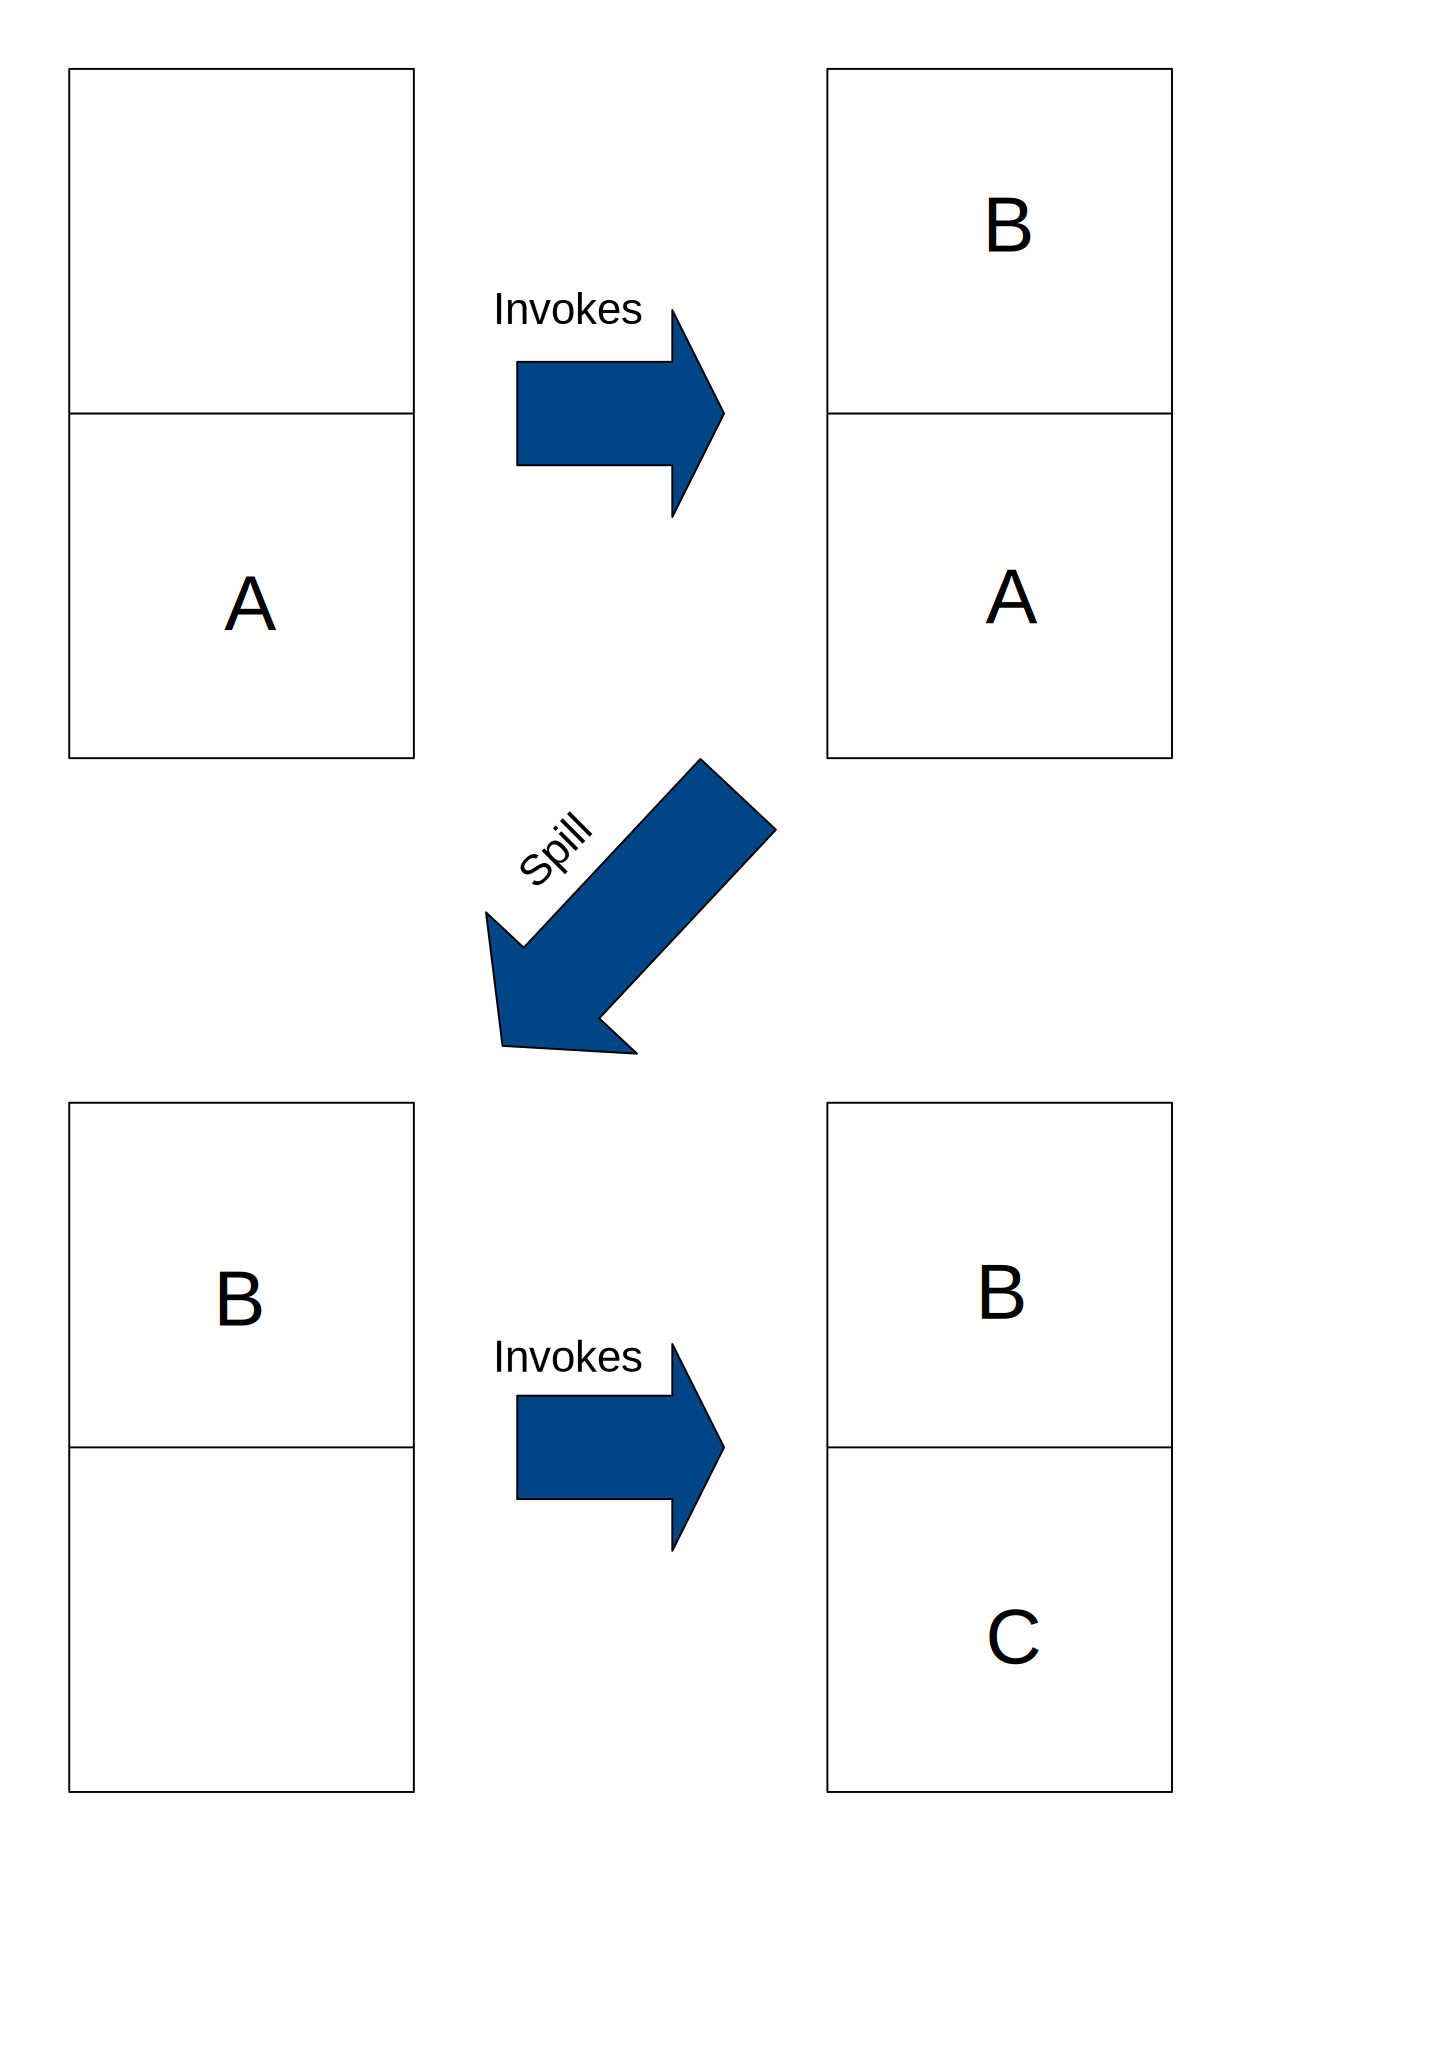
\includegraphics[height = 10cm]{PS_RS_graphics/spill.pdf}
	\caption{Spill: Verschieben des Windows }
\end{figure}

\section{Ausgelagerte Framestackteile des aktiven Threads wiederherstellen (Fill)}
Wenn der Stack durch R"uckspr"unge schrumpft und nahe dem unteren Ende des vorgehaltenen Adressbereichs kommt muss der ausgelagerte Framestack wiederhergestellt werden. 

\subsection{Ablauf eines return Vorgangs mit fill}
Im ersten Takt wird der aktuelle callercontext pointer im Register "old\_callercontext\_pointer" zwischengespeichert und es wird der Callercontext des wiederherzustellenden Stackframes ausgelesen beginnend mit den localspointer . 
Anschlie{"ss}end wird der ausgelesene localspointer gespeichert und der Stackpointer zum Auslesen adressiert. Der lokalspointer stellt das untere Ende des neuen Stackframes da. Nach dem der Stackpointer wiederhergestellt wurde wird "uberp"uft ob, der localspointer kleiner, als die unterste Adresse im Window ist, ist dies der Fall muss der Fill Vorgang gestartet werden.  
Ansonsten geht der return Vorgang normal weiter mit der Wiederherstellung des Callercontextpointers, der R"uckgabe des neuen Programmcounters "uber den AMIDAR Bus und dem aktualisieren der "Top\_of\_Stack" und "Next\_of\_Stack Register. 

\subsection {Ablauf des eigentlichen Fill Vorgangs}

Bevor das kopieren der Stackdaten passieren kann werden m"ussen die -Bottom -Top und Baseadressregister des aktuellen Windows angepasst werden. Im n"achsten Takt muss der vorher ausgelesene Programmcounter in einen Register zwischengespeichert werden, damit dieser sp"ater zur"uck gegeben werden kann. Anschlie{"ss}end wird die neue untere Adresse des Windows umgerechnet und der Lesevorgang im AXI Modul gestartet. In dem n"achsten Takt wird gewartet bis der Lesebuffer gefüllt ist. Wenn dies der Fall ist wird mit jeden weiteren Takt ein Datenwort und die dazu gehörigen Status Bits ausgelesen und von unten beginnend in das Window gespeichert. Nach jeden gespeicherten 16 Bit block wird "uberp"uft ob ein ganzes Segment "ubertragen wurde oder der ganze Burst ausgelesen wurde. Wenn ersteres der Fall ist wird der Vorgang beendet. Falls der Burst komplett "ubertragen wurde das aktuelle Segment jedoch nicht vollst"andig "ubertragen wurde wird ein neuer Leseburst mit der aktuellen Adresse gestartet. 

\begin{figure}
	\centering
	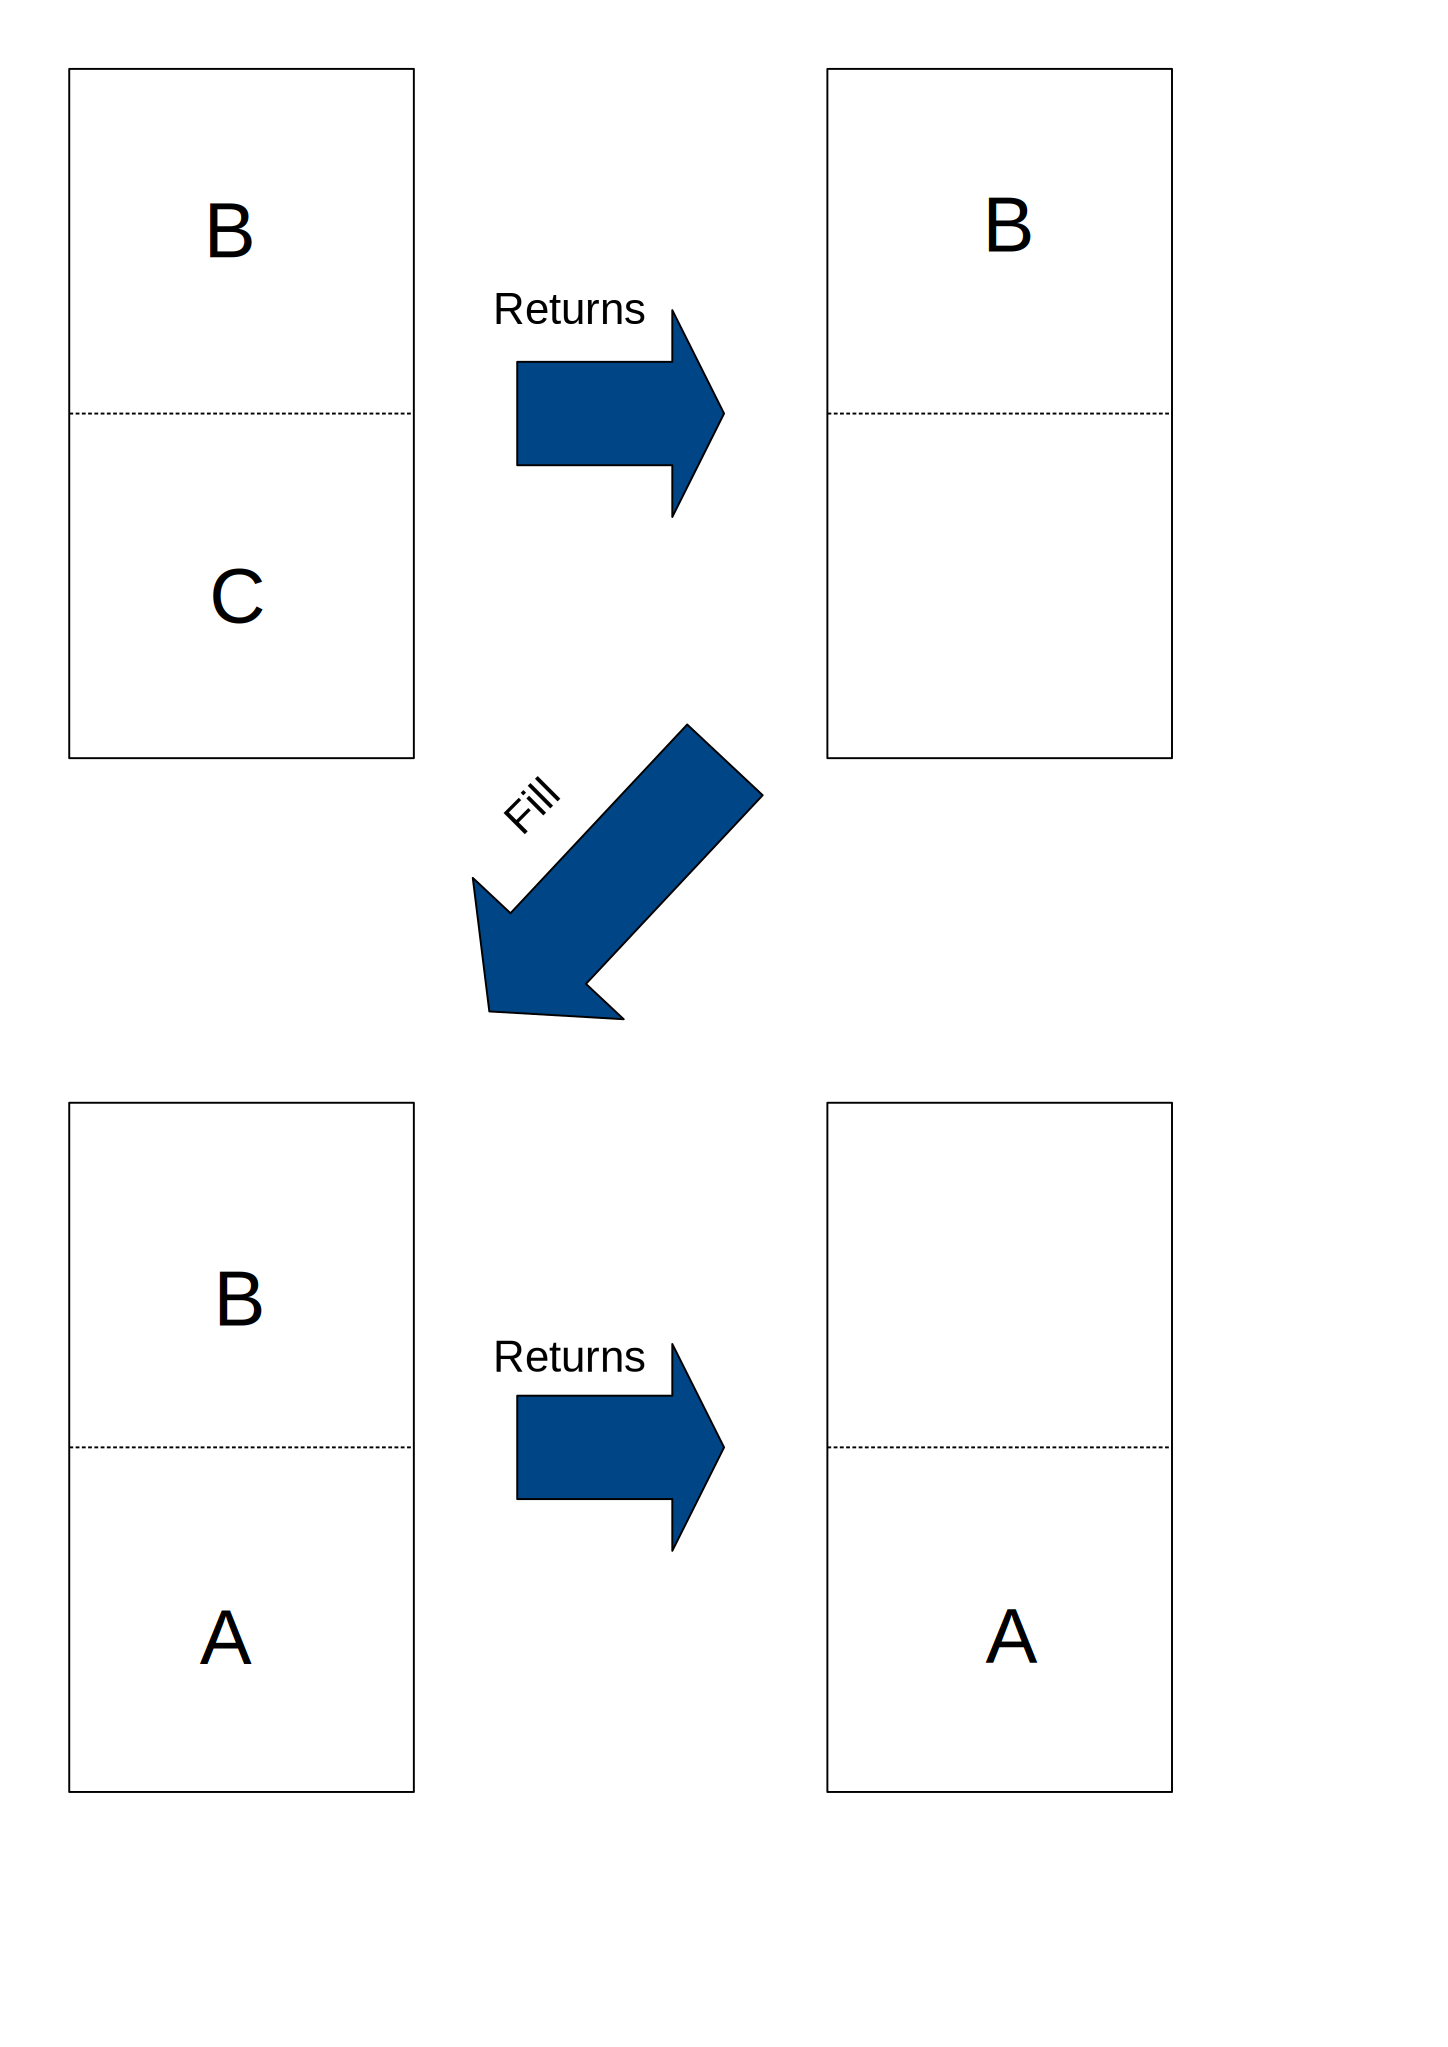
\includegraphics[height = 10cm]{PS_RS_graphics/fill.pdf}
	\caption{fill: Verschieben des Windows}
\end{figure}
\section{Multithreading mit Verdr\"angung}
Es kann eine konstante Anzahl an Threads in den Windows vorgehalten werden. Um die Multithreading Funktionalit"at mit Threads weiterhin zu gew"arleisten wurde eine Threadverdr"angung implementiert durch die Stacks von in den Hauptspeicher ausgelagert und wiederhergestellt werden k"onnen.

\subsection{Zuordnung von Threads zu den Windows}
Es gibt f"ur jedes Window ein Register in dem die zugeordnete ThreadID gespeichert wird. Dazu kommt 1 Status Bit, mit dem angegeben wird, ob dem Window bereits eine ThreadID zugeordnet ist und 4 Bits, die f"ur einen Least Recently Used counter genutzt werden. Nach einen Reset des Framestack Moduls werden alle Bits der Windows 1-n bis auf das erste Statusbit auf 0 gesetzt. F"ur Window 0, in dem der Stack des Thread 0 liegt, wird das erste Bit auf 0 gesetzt, damit es ohne explizite Threaderzeugung vom Bootloader genutzt werden kann.  


\subsection{"Anderungen am der Threaderzeugung}
Bisher wurden Threads im Framestack angelegt in dem "uber das Wishbone Interface erst der Threadtable initialisiert wird und anschlie{"ss}end der Stackframe durch Schreiben der R"ucksprungadresse und eines leeren Callercontext in den Blockram. Das Problem dabei ist durch die Auslagerung der Threads in den Framestack die Daten in den Hauptspeicher geschrieben werden m"usste, was aufwendig zu implementieren w"are und sehr viel Zeit bei der Ausf"urung ben"otigen w"urde. Es ist au{"ss}erdem nicht m"oglich neue Threads direkt im Window zu initialisieren, da es m"oglich ist das mehr Threads initialisiert werden, als Windows verf"ugbar sind, bevor die Ausf"uhrung der Threads zum ersten mal gestartet wird. 
Stattdessen wurde f"ur die Threaderzeugung der bisher ungenutzte Framestack Opcode "OP\_FRAMESTACK\_NEWTHREAD" genutzt um den Stackframe der Threads zu initialisieren. Der Threadtable wird weiterhin "uber Wishbone initialisiert. Sobald der NEWTHREAD Opcode abgearbeitet wird gepr"uft ob schon ein Thread mit der zu "uber Wishbone "ubergebenen ID in einen der Windows vorhanden ist. Ist dies der Fall wird der als Parameter mit den Opcode "ubergebene Threadhandle an Adresse 0 des entsprechenden Windows geschrieben. Dar"uber wird der Callercontext initialisiert. Wenn die ThreadID noch keinen der Windows zugewiesen ist, muss der Stackframe des Threads im externen Speicher initialisiert werden. Daf"ur wird auch das vorher beschriebene AXI Modul verwendet. Es wird der Threadhandle und der leere Callercontext "ubertragen. Au{"ss}erdem m"ussen noch 12 weitere leere W"orter "ubertragen werden um einen 16 Wort Block "ubertragen zu k"onnen. 

\subsection{Threadwechsel}
F"ur einen Threadwechsel bei einen AMIDAR Prozessor werden im Framestack die Werte der Register Stackpointer, Localspointer und Callercontext aus dem Threadtable "ubernommen. In der neuen Implementierung wird zus"atzlich gepr"uft ob, der Thread auf den gewechselt wird bereits in einen der Windows vorgehalten wird. Ist dies der Fall kann einfach auf das entsprechende Window gewechselt werden um den Thread weiter auszuf"uhren. Wenn der Stack des Threads noch nicht in einen der Windows sein sollte wird dieser aus dem Speicher geladen. Davor wird gegebenenfalls noch der Stack eines zu verdr"angender Threads in den externen Speicher vorschoben. 
\subsubsection{Ablauf des Threadwechsels}
Der Threadwechsel beginnt, wenn der Opcode "OP\_FRAMESTACK\_THREADSWITCH" abgearbeitet wird. Die ThreadID des neuen Threads wird "uber den AMIDAR-Bus "ubergeben und in einem Register gespeichert. Zu Beginn des Vorgangs wird gep"uft ob die ThreadID schon im WINDOW\_TO\_THREAD Register eingetragen ist. Ist dies nicht der Fall wird gepr"uft ob es noch ein Window leer ist. 
Wenn kein Window verf"ugbar ist werden die LRU Bits "uberpr"uft und der am wenigsten verwendete Thread bestimmt. Wenn auf einen schon vorgehaltenen Thread gewechselt wird, wird der LFU Counter des Threads um eins erh"oht. Dabei wird "uberpr"uft ob der counter des aktuellen n"achsten Threads gleich 15 ist. Ist dies der Fall wird der counter, aller Threads halbiert. 
In dem Fall, in dem ein Thread verdr"angt werden muss wird der am wenigsten verwendete Thread in den externen Speicher transferiert. Daf"ur wird die passende Burstl"ange anhand des Stackpointers und der unteren Windowadresse berechnet. Sie muss ein Vielfaches von 16 sein. Danach findet die eigentliche "Ubertragung des Stacks statt. 
Nachdem der Stackframe des zu verdr"angenden Threads gesichert wurde kann das Window mit den Stack des neuen Threads "uberschrieben werden. Daf"ur wird die untere Startadresse der "Übertragung anhand des Localspointer und der gr"o{ss}e der Windowabschnitte soda{ss} der Locals und der Stackpointer im Window liegen. Daraufhin wird der zu "ubertragende Stackframe ausgelesen und in das Window kopiert.  

\section{Garbage Collector Interface}

Der Framestack muss den Garabage Collector ein Interface zur Verf"ugung stellen "uber dass, das Rootset ausgelesen werden kann. Daf"ur werden f"ur jedes Datenwort im Framestack zwei Statusbits angegeben, die den Entrytype bescreiben. Der Entrytype 2'b10 gibt dabei Referenzen an. Um das Rootset zu erzeugen muss der Stack jedes einzelnen Threads ausgelesen werden, dabei wird bei jeden Wort gepr"uft ob der EntryType 2'b10 hinterlegt wurde, in dem Fall wird das Word an an Garbage Collector "ubertragen. Da Teile des Framestacks im externen Speicher liegen m"ussen diese ausgelesen werden.
Wenn der Eingang gc\_request\_rootset gesetzt ist beginnt der Auslese Vorgang. Der Stack wird Thread f"ur Thread ausgelesen. Nachdem ein Thread zum auslesen ausgew"ahlt wurde wird gepr"uft, ob dieser im Window liegt. Ist das der Fall wird gepr"uft, ob der komplette Stack im Window liegt. Wenn Teile des Stacks ausgelagert wurden, werden diese in 16er Bl"ocken ausgelesen und gepr"uft. Sobald die untere Grenze des Windows dabei erreicht ist, kann der Rest aus dem Window gelesen werden. Sobald alle Threads nach diesen Verfahren abgearbeitet wurden ist das Rootset komplett "ubertragen. 

\section{Lesezugriff Wishbone}
Lesezugriff "uber Wishbone auf dem Framestack musste auch umgeschrieben werden. Bisher liefen die Zugriffe direkt "uber den 2. Port des Blockram in dem der Framestack gespeichert wurde. Wegen des ausgelagerten Threads funktioniert das nur wenn die auszulesenden Daten im Window liegen. Wenn das nicht der Fall ist, m"ussen diese jeweils aus dem RAM geladen werden, was von der FramestackFSM abgearbeitet wird. W"ahrenddessen muss allerdings das Wishbone Acknowledge Signal zur"uck gehalten werden, wodurch der Wishbone-Bus eine Weile blockiert wird. Da dieser Lesezugriff nur f"ur den Debugger genutzt wird, ist die Performance bei diesen Vorgang jedoch vernachl"assigbar. 




\chapter{Evaluation}
\label{cha:Evaluation}
Um die korrekte Funktionsweise und die Performance des ge"anderten Framestacks zu "uberpr"ufen wurde eine modifizierte AMIDAR Testbench verwendet. Vorallem im Fokus stand die korrekte Ausf"uhrung der "Spill and Fill" Abl"aufe und die Threadwechsel. 
\section{Testumgebung}
F"ur die Tests wurde die AMIDAR Testbench modifiziert um Funktionen mit einen großen Framestack oder Threadwechseln zu testen. Au{ss}erdem wurde die Hardware des Framestacks erweitert um die ben"otigte Anzahl an Takten f"ur einen bestimmten Vorgang aufzuzeichnen. 
\subsection{Hardware"anderungen zur Performance Evaluation}
Um die Performance evaluieren zu k"onnen ein zus"atzlicher Blockram angelegt in dem jeweils die Dauer eines bestimmten Vorgangs protokolliert wird. Es kann entweder die Dauer der Spill, der Fill oder der Threadswitch Vorg"ange protokolliert werden. 
Um auf diese Daten zuzugreifen wurden dem Framestack die Wishbone Register 15, 16, 17 und 18 hinzugef"ufgt. Mit den Register 18 wird dabei angegeben ob und welcher Vorgang protokolliert werden soll. Wird eine 0 in das Register geschrieben wird die Protokollfunktion deaktiviert. Mit Register 15 Wird angegeben aus welcher Adresse des Speichers gelesen werden soll. Die ausgelesenen Daten selber stehen in Register 18. Das Register 17 gibt die Anzahl der Eintr"age in dem Speicher an. 
Zur Protokollierung eines Vorgans werden die Takte gez"ahlt sobald der Startzustand eines Vorgangs erreicht ist und endet wenn der Vorgang beendet wurde und neue Tokens abgearbeitet werden k"onnen. Zu beachten dabei ist, das bei jeden Vorgang nur die Anzahl der Takte gemessen wird bei denen die Framestack FSM besch"aftig ist. Beim Spill zum Beispiel wird das z"ahlen beendet sobald die letzten Stackdaten in den Schreibfifo geschrieben wurde. Die Zeit, in der der AXI Bus belegt ist, ist etwas l"anger, da der FIFO noch abgearbeitet werden muss. Der Framestack selber kann währenddessen schon weitere Token abarbeiten.
Alle eben beschriebenen "Anderungen lassen sich wenn nicht benötigt durch eine Präprozessordefinition deaktivieren. 
\subsection{angepasste Testbench}
Um die weiterhin korrekte Funktionsweise der Grundlegenden Framestack Funktionalit"aten zu testen wurde die AMIDAR Testbench genutzt. Erweitert wurde diese dabei zum einen um Tests, die den Spill and Fill Vorgang testen. Daf"ur wurde eine Funktion ben"otigt, die einen m"oglichst gro{ss}en Stack erzeugt und dennoch eine einigerma{ss}en kurze Laufzeit hat. Die Funktion zur Rekursiven Berechnung der Fibonaci Folge erzeugt zwar schnell einen sehr großen Stack, allerdings ist die Laufzeit dieser deutlich zu lang um als Test in Frage zu kommen. Zum  Testen der Spill and Fill Funktionen wurde eine vereinfachte Ackermann Funktion genutzt, die mit 2 Parametern arbeitet.
%todo code
In dem neuen Testfall AckermannTest wird diese Funktion mit unterschiedlichen Parametern aufgerufen:
Ackermann (3,3):
				Rekursionstiefe 		= 63
				Maximale Stackgr"o{ss}e = 450 Wörter
				R"uckgabewert 			= 9	
				
Ackermann (3,4):
				Rekursionstiefe			= 127
				Maximale Stackgr"o{ss}e = 890 Wörter
				R"uckgabewert			= 61

Ackermann (3,5):
				Rekursionstiefe			= 127
				Maximale Stackgr"o{ss}e = 1785 Wörter
				R"uckgabewert			= 253

Weitere wichtige Testf"alle waren die schon vorhandenen, jedoch nicht einkommentierten Multithreading Tests. Genutzt wurde der "BasicThreadTest" und der "AdvancedThreadTest". Außerdem wurde eine Modifizierte Variante des BasicThreadTests genutzt, bei der der Ackermanntest in mehreren Threads ausgef"uhrt wurde. 

Eine weitere Anpassung der Testbench ist eine Methode die "uber Wishbone die im Framestackmodul gemessenen Performancedaten ausliest.  Zuerst wird die Anzahl der erfassten Vorg"ange ausgelesen. Anschließend wird "uber den Speicher mit den Messdaten iteriert und der Inhalt ausgegeben, dabei wird das arithmetische Mittel der Messwerte berechnet und ebenfalls ausgegeben. 


\section{Performance Messungen}
\subsection{Spill}
\subsection{Fill}
\subsection{Threadswitch}

\include{Fazit}


%% Anhang %%%%%%%%%%%%%%%%%%%%%%%%%%%%%%%%%%%%%%%%%%%%%%%%%%%%%%%%%%%%%%%%
%\appendix
\bibliographystyle{plain}
\clearpage
% \nocite{*}
\bibliography{literaturverzeichnis}
\listoffigures % Abbildungsverzeichnis

\end{document}
